\section{Demonstration of Improved Decision-Making}

For our model we tried 4 different reward methods: mean of like, sum of like, mean of watch ratio, sum of watch ratio. We decided to research these four different reward methodologies because we wanted to observe how different metrics to quantify recommendations would impact our models results to effectively make recommendations. 

\subsection{Mean of Like}

\begin{figure}
    \centering
    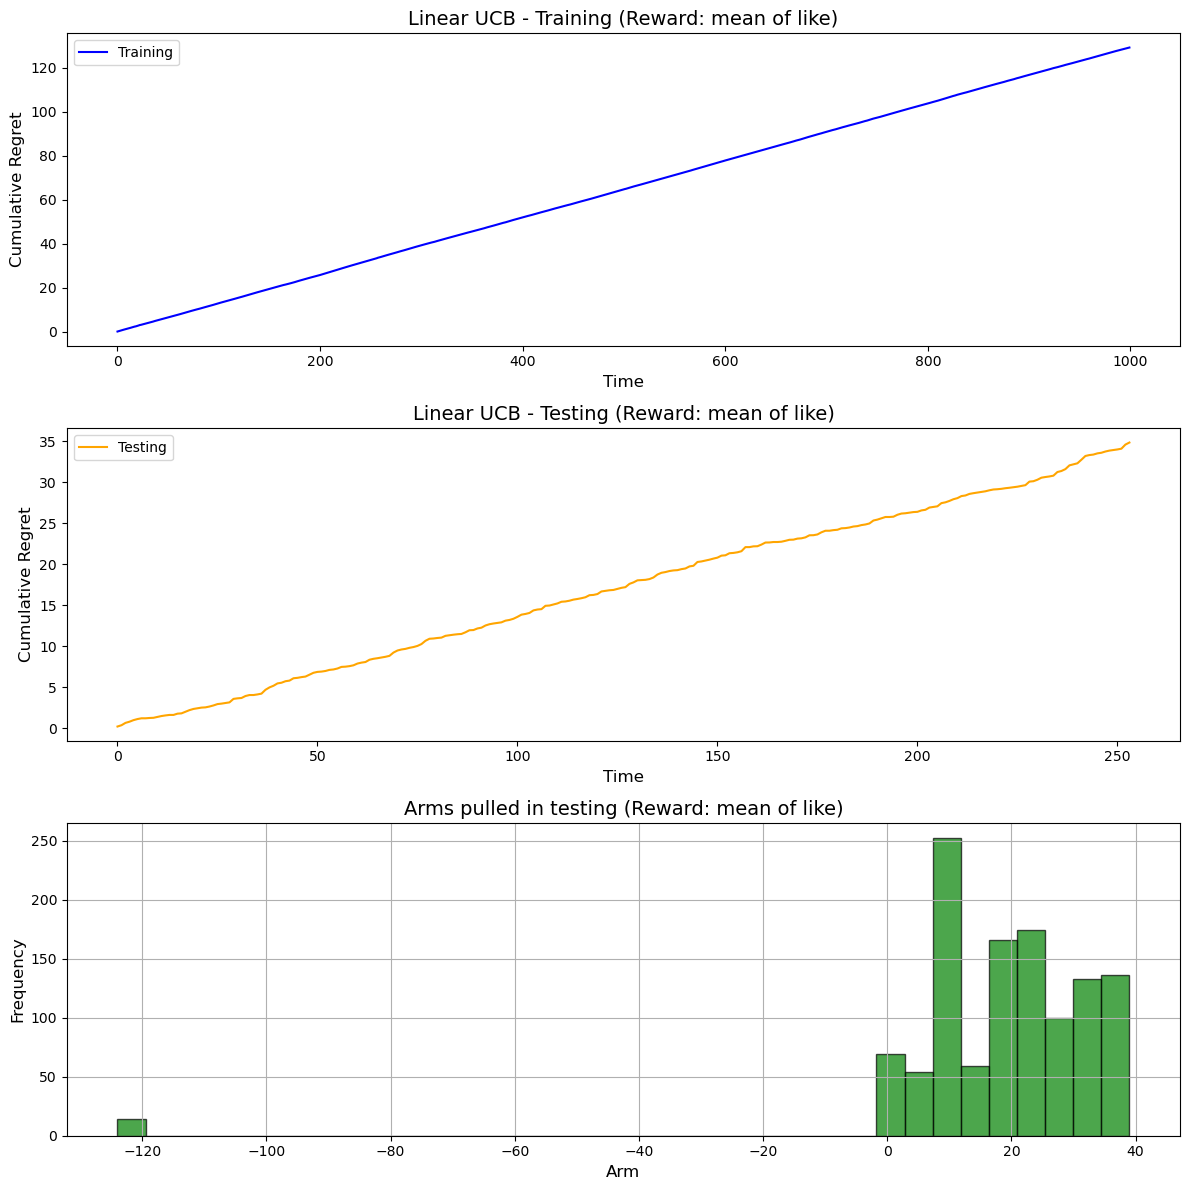
\includegraphics[width=0.5\linewidth]{mean_like.png}
    \caption{Model using mean of likes as grouping function per video category}
    \label{mean_like}
\end{figure}

The mean of like model defines each arm as the mean of likes per video category, with users the states. This model did not converge during training, as evidenced by the linear cumulative regret. In testing, the model produces a pseudo-random distribution of video category predictions \ref{mean_like}.

\subsection{Sum of Like}

\begin{figure}
    \centering
    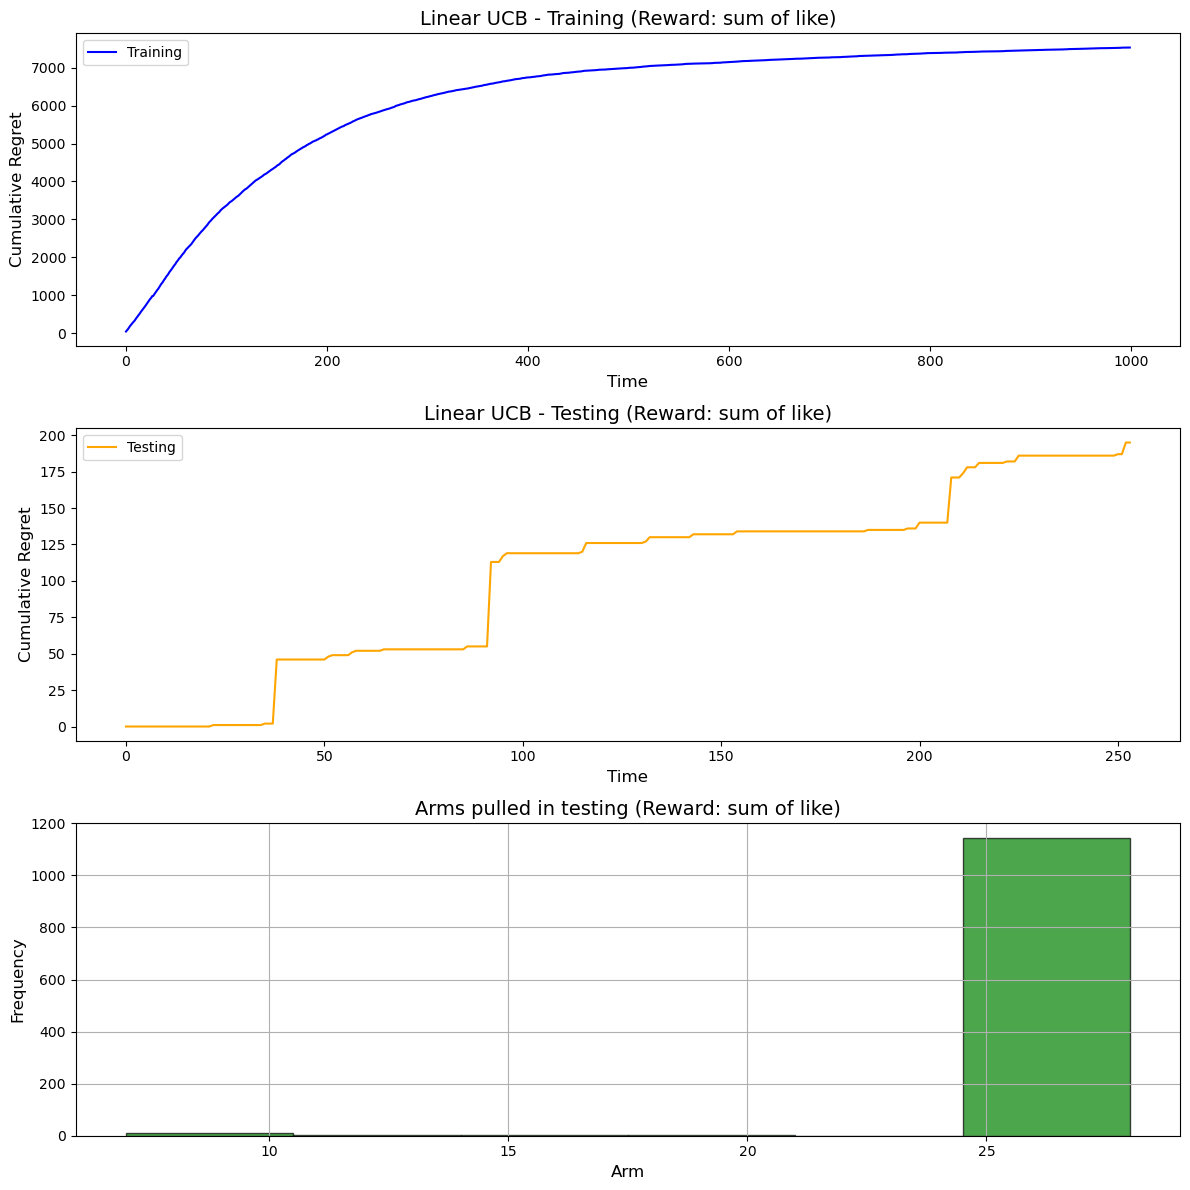
\includegraphics[width=0.5\linewidth]{sum_like.png}
    \caption{Model using sum of likes as grouping function per video category}
    \label{sum_like}
\end{figure}

The sum of like model defines each arm as the sum of likes per video category, with users the states. This model did converge during training, as evidenced by the flatting cumulative regret curve. The model generalizes poorly, however, and is heavily biased towards one arm. While the bias is heavy, the model is not completely biased and sometimes pulls non-favorite arms. This is likely due to bias in the input data, and the heavy skew of the non-normalized mean function \ref{sum_like}.

\subsection{Mean of Watch Ratio}

\begin{figure}
    \centering
    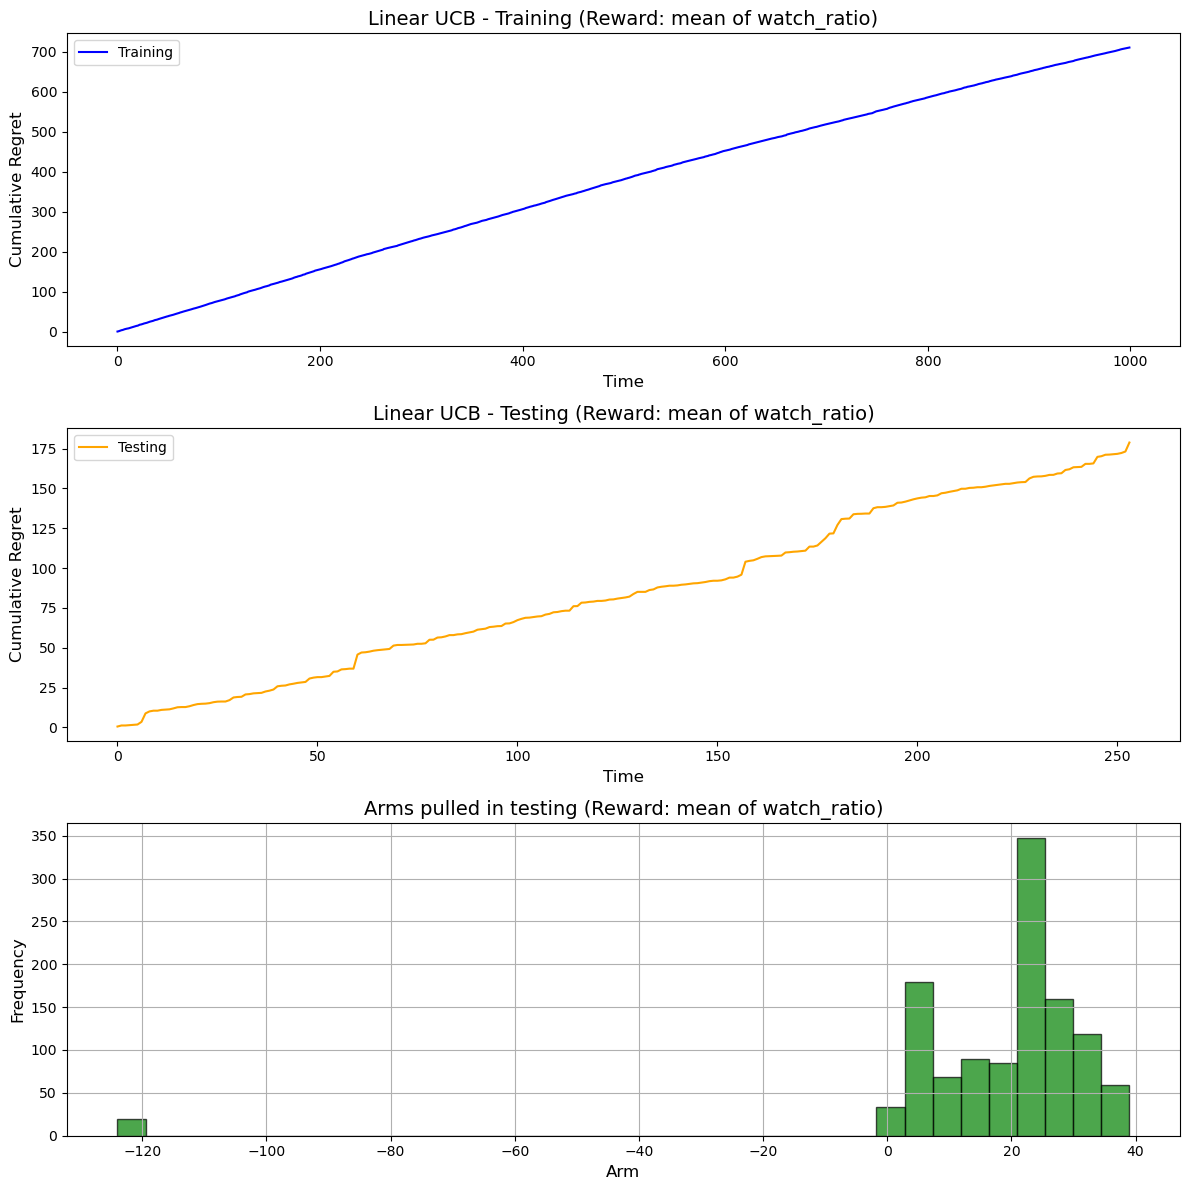
\includegraphics[width=0.5\linewidth]{mean_watchratio.png}
    \caption{Model using mean of watch ratio as grouping function per video category}
    \label{mean_watchratio}
\end{figure}

The mean of watch ratio model defines each arm as the mean of watch ratio per video category, with users the states \ref{mean_watchratio}. This model did not converge during training, as evidenced by the linear cumulative regret. In testing, the model produces a pseudo-random distribution of video category predictions, similar to the sum of like model.

\subsection{Sum of Watch Ratio}

\begin{figure}
    \centering
    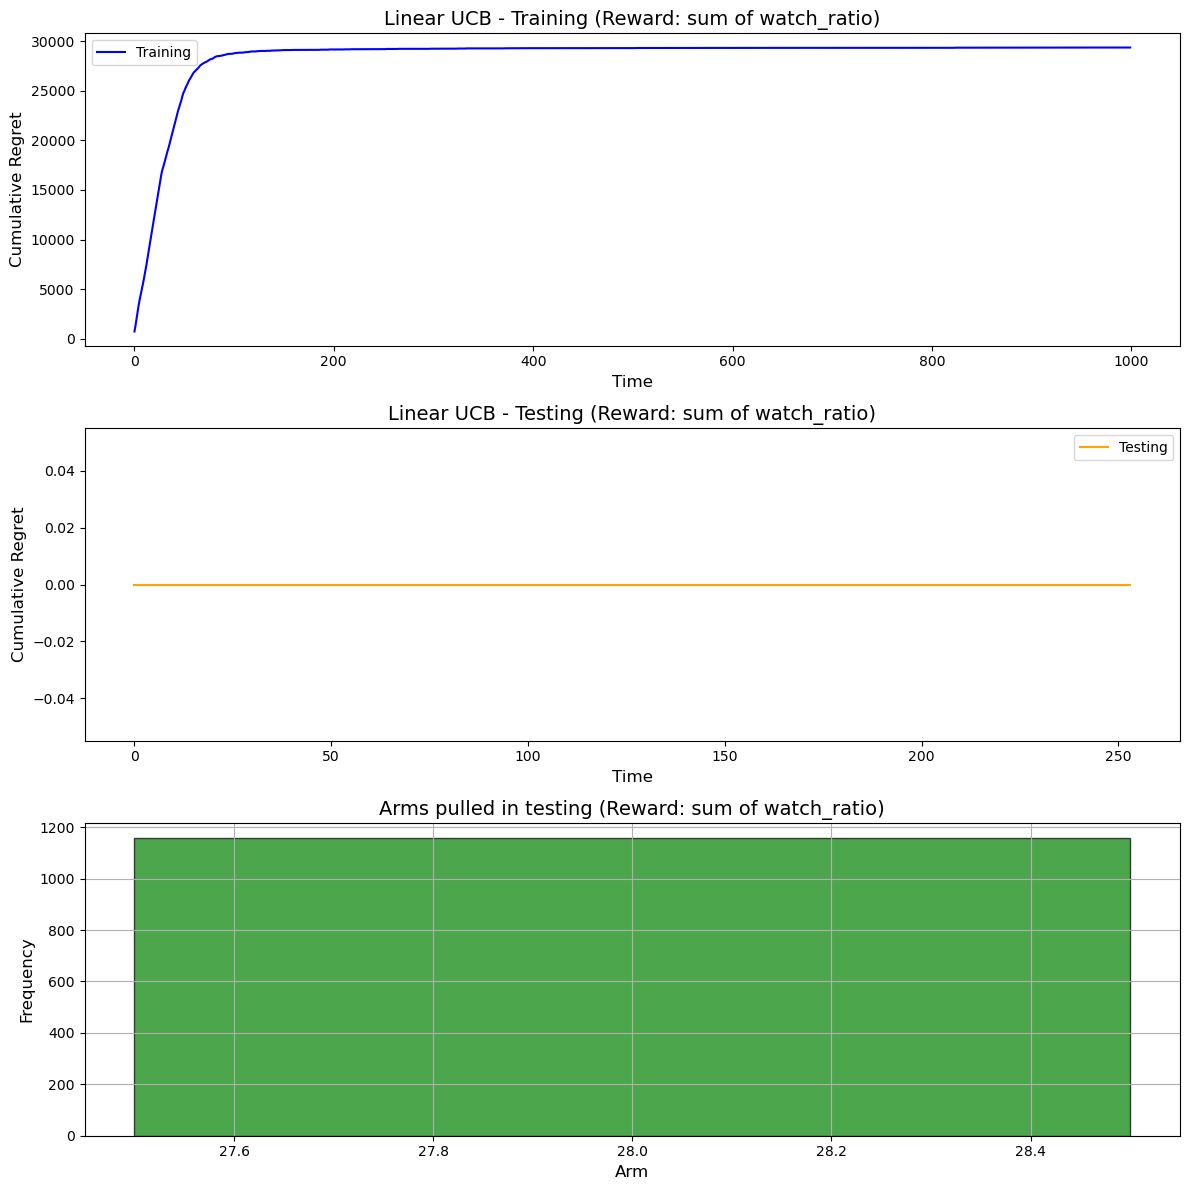
\includegraphics[width=0.5\linewidth]{summary_report/sum_watchratio.png}
    \caption{Model using sum of watch ratio as grouping function per video category}
    \label{sum_watchratio}
\end{figure}

The sum of watch ratio model defines each arm as the sum of watch ratio per video category, with users the states. This model did converge during training, as evidenced by the flatting cumulative regret curve. The model generalizes poorly, however, and is \textit{entirely} biased towards one arm. While the sum of like model sometimes pulls non-favorite arms, this model achieves 0 regret only pulling one arm, meaning there is one video category who's sum of watch ratio is higher for every user in the dataset \ref{sum_watchratio}.


% We demonstrate LinUCB's effectiveness by simulating a sequence of recommendations on the prepared KuaiRec dataset.

% \subsection{Iterative Training}

% We iteratively present users from the training set to the bandit model (Figure \ref{regret_plot}). Each user's context and available arms (categories) are fed into LinUCB. The model selects a category to recommend, observes the resulting reward (watch ratio), and updates its parameters accordingly.
    
% \subsection{Cumulative Regret Analysis}

% We measure the cumulative regret of the recommendations, defined as the difference between the reward of the chosen arm and the best possible arm in hindsight. As the model learns, the cumulative regret curve flattens, indicating that LinUCB is converging toward optimal decisions. Reduced regret over time demonstrates improved decision-making and more effective recommendations.

% \subsection{Testing and Generalization}

% After training, we apply the learned model to the test set without further parameter updates (Figure \ref{regret_plot}. By comparing cumulative regret and average rewards between the training and testing phases, we ensure that the model's performance gains are not limited to the training sample. We observe that LinUCB converges but does not generalize well. Arms 25-27 are pulled 

% The result is a recommendation strategy that adaptively learns user preferences and adjusts its recommendations to maximize engagement, all while efficiently exploring new categories that might interest users.